\documentclass[twoside]{book}

% Packages required by doxygen
\usepackage{fixltx2e}
\usepackage{calc}
\usepackage{doxygen}
\usepackage[export]{adjustbox} % also loads graphicx
\usepackage{graphicx}
\usepackage[utf8]{inputenc}
\usepackage{makeidx}
\usepackage{multicol}
\usepackage{multirow}
\PassOptionsToPackage{warn}{textcomp}
\usepackage{textcomp}
\usepackage[nointegrals]{wasysym}
\usepackage[table]{xcolor}

% Font selection
\usepackage[T1]{fontenc}
\usepackage[scaled=.90]{helvet}
\usepackage{courier}
\usepackage{amssymb}
\usepackage{sectsty}
\renewcommand{\familydefault}{\sfdefault}
\allsectionsfont{%
  \fontseries{bc}\selectfont%
  \color{darkgray}%
}
\renewcommand{\DoxyLabelFont}{%
  \fontseries{bc}\selectfont%
  \color{darkgray}%
}
\newcommand{\+}{\discretionary{\mbox{\scriptsize$\hookleftarrow$}}{}{}}

% Page & text layout
\usepackage{geometry}
\geometry{%
  a4paper,%
  top=2.5cm,%
  bottom=2.5cm,%
  left=2.5cm,%
  right=2.5cm%
}
\tolerance=750
\hfuzz=15pt
\hbadness=750
\setlength{\emergencystretch}{15pt}
\setlength{\parindent}{0cm}
\setlength{\parskip}{3ex plus 2ex minus 2ex}
\makeatletter
\renewcommand{\paragraph}{%
  \@startsection{paragraph}{4}{0ex}{-1.0ex}{1.0ex}{%
    \normalfont\normalsize\bfseries\SS@parafont%
  }%
}
\renewcommand{\subparagraph}{%
  \@startsection{subparagraph}{5}{0ex}{-1.0ex}{1.0ex}{%
    \normalfont\normalsize\bfseries\SS@subparafont%
  }%
}
\makeatother

% Headers & footers
\usepackage{fancyhdr}
\pagestyle{fancyplain}
\fancyhead[LE]{\fancyplain{}{\bfseries\thepage}}
\fancyhead[CE]{\fancyplain{}{}}
\fancyhead[RE]{\fancyplain{}{\bfseries\leftmark}}
\fancyhead[LO]{\fancyplain{}{\bfseries\rightmark}}
\fancyhead[CO]{\fancyplain{}{}}
\fancyhead[RO]{\fancyplain{}{\bfseries\thepage}}
\fancyfoot[LE]{\fancyplain{}{}}
\fancyfoot[CE]{\fancyplain{}{}}
\fancyfoot[RE]{\fancyplain{}{\bfseries\scriptsize Generated by Doxygen }}
\fancyfoot[LO]{\fancyplain{}{\bfseries\scriptsize Generated by Doxygen }}
\fancyfoot[CO]{\fancyplain{}{}}
\fancyfoot[RO]{\fancyplain{}{}}
\renewcommand{\footrulewidth}{0.4pt}
\renewcommand{\chaptermark}[1]{%
  \markboth{#1}{}%
}
\renewcommand{\sectionmark}[1]{%
  \markright{\thesection\ #1}%
}

% Indices & bibliography
\usepackage{natbib}
\usepackage[titles]{tocloft}
\setcounter{tocdepth}{3}
\setcounter{secnumdepth}{5}
\makeindex

% Hyperlinks (required, but should be loaded last)
\usepackage{ifpdf}
\ifpdf
  \usepackage[pdftex,pagebackref=true]{hyperref}
\else
  \usepackage[ps2pdf,pagebackref=true]{hyperref}
\fi
\hypersetup{%
  colorlinks=true,%
  linkcolor=blue,%
  citecolor=blue,%
  unicode%
}

% Custom commands
\newcommand{\clearemptydoublepage}{%
  \newpage{\pagestyle{empty}\cleardoublepage}%
}

\usepackage{caption}
\captionsetup{labelsep=space,justification=centering,font={bf},singlelinecheck=off,skip=4pt,position=top}

%===== C O N T E N T S =====

\begin{document}

% Titlepage & ToC
\hypersetup{pageanchor=false,
             bookmarksnumbered=true,
             pdfencoding=unicode
            }
\pagenumbering{roman}
\begin{titlepage}
\vspace*{7cm}
\begin{center}%
{\Large Mind\+Engine }\\
\vspace*{1cm}
{\large Generated by Doxygen 1.8.11}\\
\end{center}
\end{titlepage}
\clearemptydoublepage
\tableofcontents
\clearemptydoublepage
\pagenumbering{arabic}
\hypersetup{pageanchor=true}

%--- Begin generated contents ---
\chapter{Todo List}
\label{todo}
\hypertarget{todo}{}

\begin{DoxyRefList}
\item[\label{todo__todo000001}%
\hypertarget{todo__todo000001}{}%
Member \hyperlink{classDatabase_1_1DataNode_ace59a7fba9c490d2dae59c4af7b0c71f}{Database\+:\+:Data\+Node\+:\+:identifier} ]Use identifier with strings may decrease performance with large systems due to string-\/matching operations. Will change this to integer or unsigned integer as soon as I find a way to match identifier with human-\/readable strings.  
\item[\label{todo__todo000002}%
\hypertarget{todo__todo000002}{}%
Member \hyperlink{classRules_1_1Rule_a6fe9b4fa6aaface7ba7f2400d2b27dbc}{Rules\+:\+:Rule\+:\+:action} ()=0]Examine the performance and reusability of using a method. If it is hard to expand, find a way to use a struct/class instead. 
\end{DoxyRefList}
\chapter{Namespace Index}
\section{Namespace List}
Here is a list of all documented namespaces with brief descriptions\+:\begin{DoxyCompactList}
\item\contentsline{section}{\hyperlink{namespaceDatabase}{Database} \\*The \hyperlink{namespaceDatabase}{Database} namespace }{\pageref{namespaceDatabase}}{}
\end{DoxyCompactList}

\chapter{Hierarchical Index}
\section{Class Hierarchy}
This inheritance list is sorted roughly, but not completely, alphabetically\+:\begin{DoxyCompactList}
\item \contentsline{section}{Database\+:\+:Data\+Node}{\pageref{classDatabase_1_1DataNode}}{}
\begin{DoxyCompactList}
\item \contentsline{section}{Database\+:\+:Data\+Group}{\pageref{classDatabase_1_1DataGroup}}{}
\end{DoxyCompactList}
\item \contentsline{section}{Database\+:\+:Datum$<$ T $>$}{\pageref{classDatabase_1_1Datum}}{}
\end{DoxyCompactList}

\chapter{Class Index}
\section{Class List}
Here are the classes, structs, unions and interfaces with brief descriptions\+:\begin{DoxyCompactList}
\item\contentsline{section}{\hyperlink{classDatabase_1_1DataGroup}{Database\+::\+Data\+Group} \\*The \hyperlink{classDatabase_1_1DataGroup}{Data\+Group} class Represents a non-\/leaf node, which contains children. Its children can be any \hyperlink{classDatabase_1_1DataNode}{Data\+Node} object\+: either another data group, or a datum only }{\pageref{classDatabase_1_1DataGroup}}{}
\item\contentsline{section}{\hyperlink{classDatabase_1_1DataNode}{Database\+::\+Data\+Node} \\*The \hyperlink{classDatabase_1_1DataNode}{Data\+Node} class Base class of each node in the database tree. Since every node needs an identifier, but non-\/leaf nodes contain their children, while leaf nodes store values }{\pageref{classDatabase_1_1DataNode}}{}
\item\contentsline{section}{\hyperlink{classDatabase_1_1Datum}{Database\+::\+Datum$<$ T $>$} \\*The \hyperlink{classDatabase_1_1Datum}{Datum} class A \hyperlink{classDatabase_1_1Datum}{Datum} consists of an identifier and and value. In \hyperlink{namespaceDatabase}{Database}\textquotesingle{}s tree structure, a leaf node is a \hyperlink{classDatabase_1_1Datum}{Datum} }{\pageref{classDatabase_1_1Datum}}{}
\end{DoxyCompactList}

\chapter{Namespace Documentation}
\hypertarget{namespaceDatabase}{}\section{Database Namespace Reference}
\label{namespaceDatabase}\index{Database@{Database}}


Contains classes to represent Rule-\/based system\textquotesingle{}s database, which stores knowledge available to the AI agent.  


\subsection*{Classes}
\begin{DoxyCompactItemize}
\item 
class \hyperlink{classDatabase_1_1DataGroup}{Data\+Group}
\begin{DoxyCompactList}\small\item\em Represents a non-\/leaf node, which contains children. Its children can be any \hyperlink{classDatabase_1_1DataNode}{Data\+Node} object\+: either another \hyperlink{classDatabase_1_1DataGroup}{Data\+Group}, or a \hyperlink{classDatabase_1_1Datum}{Datum} only. \end{DoxyCompactList}\item 
class \hyperlink{classDatabase_1_1DataNode}{Data\+Node}
\begin{DoxyCompactList}\small\item\em Base class of each node in the database tree. Since every node needs an identifier, but non-\/leaf nodes contain their children, while leaf nodes store values. \end{DoxyCompactList}\item 
class \hyperlink{classDatabase_1_1Datum}{Datum}
\begin{DoxyCompactList}\small\item\em A \hyperlink{classDatabase_1_1Datum}{Datum} consists of an identifier and and value. In \hyperlink{namespaceDatabase}{Database}\textquotesingle{}s tree structure, a leaf node is a \hyperlink{classDatabase_1_1Datum}{Datum}. \end{DoxyCompactList}\end{DoxyCompactItemize}


\subsection{Detailed Description}
Contains classes to represent Rule-\/based system\textquotesingle{}s database, which stores knowledge available to the AI agent. 
\hypertarget{namespaceRules}{}\section{Rules Namespace Reference}
\label{namespaceRules}\index{Rules@{Rules}}


Contains the implementation of rules as well as the mechanism to match the rules and the data in the database.  


\subsection*{Classes}
\begin{DoxyCompactItemize}
\item 
struct \hyperlink{structRules_1_1Match}{Match}
\begin{DoxyCompactList}\small\item\em Provides the mechanism to match the data item from the rule with any item inside the database. \end{DoxyCompactList}\item 
class \hyperlink{classRules_1_1Rule}{Rule}
\begin{DoxyCompactList}\small\item\em Represent a rule in a Rule-\/based system. A rule has two components\+: an if clause is going to be used to match against the database and a function to perform any action required. \end{DoxyCompactList}\end{DoxyCompactItemize}


\subsection{Detailed Description}
Contains the implementation of rules as well as the mechanism to match the rules and the data in the database. 
\chapter{Class Documentation}
\hypertarget{classDatabase_1_1DataGroup}{}\section{Database\+:\+:Data\+Group Class Reference}
\label{classDatabase_1_1DataGroup}\index{Database\+::\+Data\+Group@{Database\+::\+Data\+Group}}


The \hyperlink{classDatabase_1_1DataGroup}{Data\+Group} class Represents a non-\/leaf node, which contains children. Its children can be any \hyperlink{classDatabase_1_1DataNode}{Data\+Node} object\+: either another \hyperlink{classDatabase_1_1DataGroup}{Data\+Group}, or a \hyperlink{classDatabase_1_1Datum}{Datum} only.  




{\ttfamily \#include $<$Data\+Group.\+h$>$}

Inheritance diagram for Database\+:\+:Data\+Group\+:\begin{figure}[H]
\begin{center}
\leavevmode
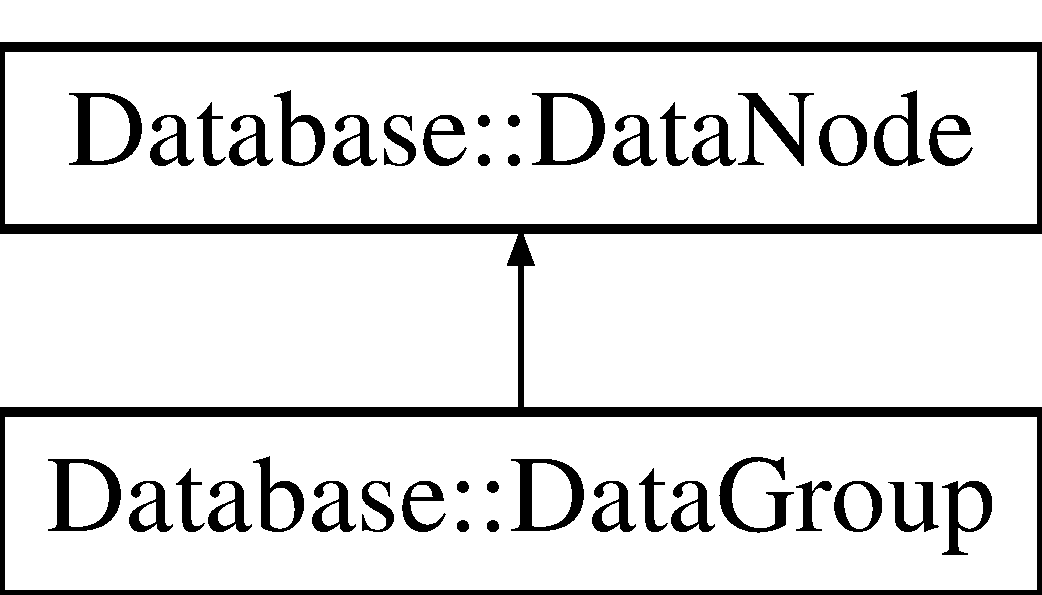
\includegraphics[height=2.000000cm]{classDatabase_1_1DataGroup}
\end{center}
\end{figure}
\subsection*{Public Member Functions}
\begin{DoxyCompactItemize}
\item 
\hyperlink{classDatabase_1_1DataGroup_a633bd46aaee7adafcb0181b12c2466f0}{Data\+Group} ()\hypertarget{classDatabase_1_1DataGroup_a633bd46aaee7adafcb0181b12c2466f0}{}\label{classDatabase_1_1DataGroup_a633bd46aaee7adafcb0181b12c2466f0}

\begin{DoxyCompactList}\small\item\em \hyperlink{classDatabase_1_1DataGroup}{Data\+Group} default constructor. \end{DoxyCompactList}\item 
\hyperlink{classDatabase_1_1DataGroup_a1bed40d80c81f52145c4696b7c70d75b}{Data\+Group} (const std\+::string \&\hyperlink{classDatabase_1_1DataNode_ace59a7fba9c490d2dae59c4af7b0c71f}{identifier}, \hyperlink{classDatabase_1_1DataNode}{Data\+Node} $\ast$\hyperlink{classDatabase_1_1DataNode_a8d70472d0f14aa3ae3ee74d9f3e879d6}{parent}, \hyperlink{classDatabase_1_1DataNode}{Data\+Node} $\ast$\hyperlink{classDatabase_1_1DataNode_ae335fc33c3813e8a6638d50faef44d5d}{right\+Sibling}, \hyperlink{classDatabase_1_1DataNode}{Data\+Node} $\ast$left\+Most\+Child)
\begin{DoxyCompactList}\small\item\em \hyperlink{classDatabase_1_1DataGroup}{Data\+Group} constructor. \end{DoxyCompactList}\item 
virtual \hyperlink{classDatabase_1_1DataGroup_a88b36fe397284004ce86726e7808466e}{$\sim$\+Data\+Group} ()\hypertarget{classDatabase_1_1DataGroup_a88b36fe397284004ce86726e7808466e}{}\label{classDatabase_1_1DataGroup_a88b36fe397284004ce86726e7808466e}

\begin{DoxyCompactList}\small\item\em $\sim$\+Data\+Group destructor \end{DoxyCompactList}\item 
const \hyperlink{classDatabase_1_1DataNode}{Data\+Node} $\ast$ \hyperlink{classDatabase_1_1DataGroup_af6abab9878250ade850fc8e43042ab01}{get\+Left\+Most\+Child} ()
\begin{DoxyCompactList}\small\item\em get\+Left\+Most\+Child \end{DoxyCompactList}\end{DoxyCompactItemize}
\subsection*{Additional Inherited Members}


\subsection{Detailed Description}
The \hyperlink{classDatabase_1_1DataGroup}{Data\+Group} class Represents a non-\/leaf node, which contains children. Its children can be any \hyperlink{classDatabase_1_1DataNode}{Data\+Node} object\+: either another \hyperlink{classDatabase_1_1DataGroup}{Data\+Group}, or a \hyperlink{classDatabase_1_1Datum}{Datum} only. 

\begin{DoxySeeAlso}{See also}
\hyperlink{classDatabase_1_1DataNode}{Data\+Node} 

\hyperlink{classDatabase_1_1Datum}{Datum} 
\end{DoxySeeAlso}


\subsection{Constructor \& Destructor Documentation}
\index{Database\+::\+Data\+Group@{Database\+::\+Data\+Group}!Data\+Group@{Data\+Group}}
\index{Data\+Group@{Data\+Group}!Database\+::\+Data\+Group@{Database\+::\+Data\+Group}}
\subsubsection[{\texorpdfstring{Data\+Group(const std\+::string \&identifier, Data\+Node $\ast$parent, Data\+Node $\ast$right\+Sibling, Data\+Node $\ast$left\+Most\+Child)}{DataGroup(const std::string &identifier, DataNode *parent, DataNode *rightSibling, DataNode *leftMostChild)}}]{\setlength{\rightskip}{0pt plus 5cm}Database\+::\+Data\+Group\+::\+Data\+Group (
\begin{DoxyParamCaption}
\item[{const std\+::string \&}]{identifier, }
\item[{{\bf Data\+Node} $\ast$}]{parent, }
\item[{{\bf Data\+Node} $\ast$}]{right\+Sibling, }
\item[{{\bf Data\+Node} $\ast$}]{left\+Most\+Child}
\end{DoxyParamCaption}
)}\hypertarget{classDatabase_1_1DataGroup_a1bed40d80c81f52145c4696b7c70d75b}{}\label{classDatabase_1_1DataGroup_a1bed40d80c81f52145c4696b7c70d75b}


\hyperlink{classDatabase_1_1DataGroup}{Data\+Group} constructor. 


\begin{DoxyParams}{Parameters}
{\em identifier} & a string parameter \\
\hline
{\em parent} & a \hyperlink{classDatabase_1_1DataNode}{Data\+Node} pointer representing this node\textquotesingle{}s parent in tree structure \\
\hline
{\em right\+Sibling} & a \hyperlink{classDatabase_1_1DataNode}{Data\+Node} pointer representing this node\textquotesingle{}s right sibling in tree \\
\hline
{\em left\+Most\+Child} & a \hyperlink{classDatabase_1_1DataNode}{Data\+Node} pointer representing this node\textquotesingle{}s left most child in tree \\
\hline
\end{DoxyParams}


\subsection{Member Function Documentation}
\index{Database\+::\+Data\+Group@{Database\+::\+Data\+Group}!get\+Left\+Most\+Child@{get\+Left\+Most\+Child}}
\index{get\+Left\+Most\+Child@{get\+Left\+Most\+Child}!Database\+::\+Data\+Group@{Database\+::\+Data\+Group}}
\subsubsection[{\texorpdfstring{get\+Left\+Most\+Child()}{getLeftMostChild()}}]{\setlength{\rightskip}{0pt plus 5cm}const {\bf Data\+Node} $\ast$ Database\+::\+Data\+Group\+::get\+Left\+Most\+Child (
\begin{DoxyParamCaption}
{}
\end{DoxyParamCaption}
)}\hypertarget{classDatabase_1_1DataGroup_af6abab9878250ade850fc8e43042ab01}{}\label{classDatabase_1_1DataGroup_af6abab9878250ade850fc8e43042ab01}


get\+Left\+Most\+Child 

\begin{DoxyReturn}{Returns}
The left most child of this data group node 
\end{DoxyReturn}


The documentation for this class was generated from the following files\+:\begin{DoxyCompactItemize}
\item 
Engine/\+Database/Data\+Group.\+h\item 
Engine/\+Database/Data\+Group.\+cpp\end{DoxyCompactItemize}

\hypertarget{structRules_1_1DataGroupMatch}{}\section{Rules\+:\+:Data\+Group\+Match Struct Reference}
\label{structRules_1_1DataGroupMatch}\index{Rules\+::\+Data\+Group\+Match@{Rules\+::\+Data\+Group\+Match}}


Matches a group of data in the database. This is done by building a match data structure that mirrors the data structure that is being searched for in the database.  




{\ttfamily \#include $<$Data\+Group\+Match.\+h$>$}

\subsection*{Public Member Functions}
\begin{DoxyCompactItemize}
\item 
virtual bool \hyperlink{structRules_1_1DataGroupMatch_afe0f2d2d965ead95d330095591b9d830}{matches\+Node} (const \hyperlink{classDatabase_1_1DataNode}{Database\+::\+Data\+Node} $\ast$node, void $\ast$bindings)
\begin{DoxyCompactList}\small\item\em Tries to match the given data node from the database against the criteria. Method used\+: a recursive matching algorithm that travels down the given node, trying to match it against the structure of this match and its children. \end{DoxyCompactList}\end{DoxyCompactItemize}
\subsection*{Public Attributes}
\begin{DoxyCompactItemize}
\item 
\hyperlink{namespaceDatabase_abca840aa37b2fd02e1d82e32a8171437}{Database\+::\+Id\+Type} \hyperlink{structRules_1_1DataGroupMatch_a8ff473135e5a803c36cd8b2b23296da3}{identifier}\hypertarget{structRules_1_1DataGroupMatch_a8ff473135e5a803c36cd8b2b23296da3}{}\label{structRules_1_1DataGroupMatch_a8ff473135e5a803c36cd8b2b23296da3}

\begin{DoxyCompactList}\small\item\em The identifier to match. \end{DoxyCompactList}\item 
\hyperlink{structRules_1_1DataNodeMatch}{Data\+Node\+Match} $\ast$ \hyperlink{structRules_1_1DataGroupMatch_a3dd32fca397944ef759c6f236548077a}{left\+Most\+Child}\hypertarget{structRules_1_1DataGroupMatch_a3dd32fca397944ef759c6f236548077a}{}\label{structRules_1_1DataGroupMatch_a3dd32fca397944ef759c6f236548077a}

\begin{DoxyCompactList}\small\item\em The first sub-\/match in this group. \end{DoxyCompactList}\end{DoxyCompactItemize}


\subsection{Detailed Description}
Matches a group of data in the database. This is done by building a match data structure that mirrors the data structure that is being searched for in the database. 

\subsection{Member Function Documentation}
\index{Rules\+::\+Data\+Group\+Match@{Rules\+::\+Data\+Group\+Match}!matches\+Node@{matches\+Node}}
\index{matches\+Node@{matches\+Node}!Rules\+::\+Data\+Group\+Match@{Rules\+::\+Data\+Group\+Match}}
\subsubsection[{\texorpdfstring{matches\+Node(const Database\+::\+Data\+Node $\ast$node, void $\ast$bindings)}{matchesNode(const Database::DataNode *node, void *bindings)}}]{\setlength{\rightskip}{0pt plus 5cm}bool Rules\+::\+Data\+Group\+Match\+::matches\+Node (
\begin{DoxyParamCaption}
\item[{const {\bf Database\+::\+Data\+Node} $\ast$}]{node, }
\item[{void $\ast$}]{bindings}
\end{DoxyParamCaption}
)\hspace{0.3cm}{\ttfamily [virtual]}}\hypertarget{structRules_1_1DataGroupMatch_afe0f2d2d965ead95d330095591b9d830}{}\label{structRules_1_1DataGroupMatch_afe0f2d2d965ead95d330095591b9d830}


Tries to match the given data node from the database against the criteria. Method used\+: a recursive matching algorithm that travels down the given node, trying to match it against the structure of this match and its children. 


\begin{DoxyParams}{Parameters}
{\em node} & The database to match on. \\
\hline
{\em bindings} & When part of the if clause matches a wild card, it is added to the bindings. This parameter is both input and output parameter. \\
\hline
\end{DoxyParams}
\begin{DoxyReturn}{Returns}
true if matches, otherwise return false. 
\end{DoxyReturn}
\begin{DoxyRefDesc}{Todo}
\item[\hyperlink{todo__todo000002}{Todo}]Add check for wildcard identifier with strings. \end{DoxyRefDesc}


\begin{DoxyRefDesc}{Todo}
\item[\hyperlink{todo__todo000003}{Todo}]Add check for wildcards here. \end{DoxyRefDesc}


The documentation for this struct was generated from the following files\+:\begin{DoxyCompactItemize}
\item 
Engine/\+Rules/Data\+Group\+Match.\+h\item 
Engine/\+Rules/Data\+Group\+Match.\+cpp\end{DoxyCompactItemize}

\hypertarget{classDatabase_1_1DataNode}{}\section{Database\+:\+:Data\+Node Class Reference}
\label{classDatabase_1_1DataNode}\index{Database\+::\+Data\+Node@{Database\+::\+Data\+Node}}


Base class of each node in the database tree. Since every node needs an identifier, but non-\/leaf nodes contain their children, while leaf nodes store values.  




{\ttfamily \#include $<$Data\+Node.\+h$>$}

Inheritance diagram for Database\+:\+:Data\+Node\+:\begin{figure}[H]
\begin{center}
\leavevmode
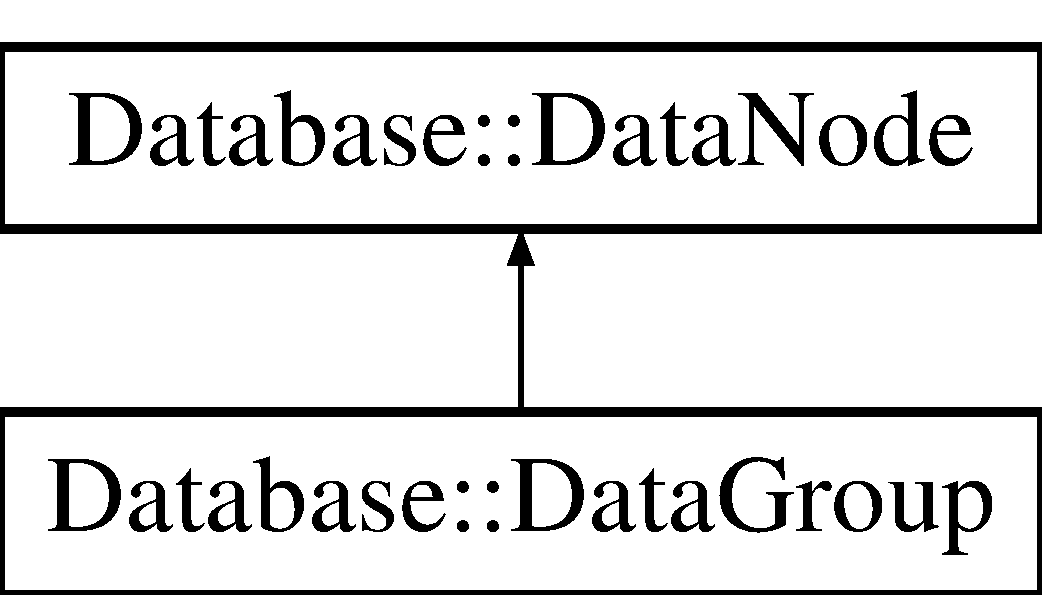
\includegraphics[height=2.000000cm]{classDatabase_1_1DataNode}
\end{center}
\end{figure}
\subsection*{Public Member Functions}
\begin{DoxyCompactItemize}
\item 
\hyperlink{classDatabase_1_1DataNode_a7999f782bb0465613e703364db8cd22a}{Data\+Node} ()\hypertarget{classDatabase_1_1DataNode_a7999f782bb0465613e703364db8cd22a}{}\label{classDatabase_1_1DataNode_a7999f782bb0465613e703364db8cd22a}

\begin{DoxyCompactList}\small\item\em \hyperlink{classDatabase_1_1DataNode}{Data\+Node} default constructor. \end{DoxyCompactList}\item 
\hyperlink{classDatabase_1_1DataNode_ae5b8832fbaf844bd74739bb7d1ce6737}{Data\+Node} (const \hyperlink{namespaceDatabase_abca840aa37b2fd02e1d82e32a8171437}{Id\+Type} \&\hyperlink{classDatabase_1_1DataNode_a2417b60924a11cf9157b996fbf7b2ca5}{identifier}, \hyperlink{classDatabase_1_1DataNode}{Data\+Node} $\ast$\hyperlink{classDatabase_1_1DataNode_ae335fc33c3813e8a6638d50faef44d5d}{right\+Sibling})
\begin{DoxyCompactList}\small\item\em \hyperlink{classDatabase_1_1DataNode}{Data\+Node} constructor with parameters. \end{DoxyCompactList}\item 
virtual \hyperlink{classDatabase_1_1DataNode_ac58f04cb07497c0b0028398f18f36c4f}{$\sim$\+Data\+Node} ()\hypertarget{classDatabase_1_1DataNode_ac58f04cb07497c0b0028398f18f36c4f}{}\label{classDatabase_1_1DataNode_ac58f04cb07497c0b0028398f18f36c4f}

\begin{DoxyCompactList}\small\item\em $\sim$\+Data\+Node destructor. \end{DoxyCompactList}\item 
\hyperlink{namespaceDatabase_abca840aa37b2fd02e1d82e32a8171437}{Id\+Type} \hyperlink{classDatabase_1_1DataNode_a09dc909b1f926bb3cedb4b383d73abe0}{get\+Identifier} () const 
\begin{DoxyCompactList}\small\item\em The data nodes have unique identifiers. \end{DoxyCompactList}\item 
\hyperlink{classDatabase_1_1DataNode}{Data\+Node} $\ast$ \hyperlink{classDatabase_1_1DataNode_a6a947c91feca4c555c4f5f0197b232ab}{get\+Right\+Sibling} () const 
\begin{DoxyCompactList}\small\item\em Data nodes are put into a left-\/most child, right sibling tree. This function is used to get the sibling next to current node. \end{DoxyCompactList}\item 
virtual bool \hyperlink{classDatabase_1_1DataNode_acba6b71939d41a2b88a9e521788033f4}{is\+Group} () const 
\begin{DoxyCompactList}\small\item\em Allows user to check whether this node is a \hyperlink{classDatabase_1_1DataGroup}{Data\+Group} or not. \end{DoxyCompactList}\item 
virtual bool \hyperlink{classDatabase_1_1DataNode_aaaef3938872f97819ed1c160c74c97cc}{is\+Datum} () const 
\begin{DoxyCompactList}\small\item\em Allows user to check whether this node is a \hyperlink{classDatabase_1_1Datum}{Datum} or not. \end{DoxyCompactList}\end{DoxyCompactItemize}
\subsection*{Protected Attributes}
\begin{DoxyCompactItemize}
\item 
\hyperlink{namespaceDatabase_abca840aa37b2fd02e1d82e32a8171437}{Id\+Type} \hyperlink{classDatabase_1_1DataNode_a2417b60924a11cf9157b996fbf7b2ca5}{identifier}\hypertarget{classDatabase_1_1DataNode_a2417b60924a11cf9157b996fbf7b2ca5}{}\label{classDatabase_1_1DataNode_a2417b60924a11cf9157b996fbf7b2ca5}

\begin{DoxyCompactList}\small\item\em Each item of data should be identified to know what the value means. \end{DoxyCompactList}\item 
\hyperlink{classDatabase_1_1DataNode}{Data\+Node} $\ast$ \hyperlink{classDatabase_1_1DataNode_ae335fc33c3813e8a6638d50faef44d5d}{right\+Sibling}\hypertarget{classDatabase_1_1DataNode_ae335fc33c3813e8a6638d50faef44d5d}{}\label{classDatabase_1_1DataNode_ae335fc33c3813e8a6638d50faef44d5d}

\begin{DoxyCompactList}\small\item\em The right sibling node of this node, or N\+U\+LL if this node is the right most child. \end{DoxyCompactList}\end{DoxyCompactItemize}


\subsection{Detailed Description}
Base class of each node in the database tree. Since every node needs an identifier, but non-\/leaf nodes contain their children, while leaf nodes store values. 

\begin{DoxySeeAlso}{See also}
\hyperlink{classDatabase_1_1DataGroup}{Data\+Group} 

\hyperlink{classDatabase_1_1Datum}{Datum} 
\end{DoxySeeAlso}


\subsection{Constructor \& Destructor Documentation}
\index{Database\+::\+Data\+Node@{Database\+::\+Data\+Node}!Data\+Node@{Data\+Node}}
\index{Data\+Node@{Data\+Node}!Database\+::\+Data\+Node@{Database\+::\+Data\+Node}}
\subsubsection[{\texorpdfstring{Data\+Node(const Id\+Type \&identifier, Data\+Node $\ast$right\+Sibling)}{DataNode(const IdType &identifier, DataNode *rightSibling)}}]{\setlength{\rightskip}{0pt plus 5cm}Database\+::\+Data\+Node\+::\+Data\+Node (
\begin{DoxyParamCaption}
\item[{const {\bf Id\+Type} \&}]{identifier, }
\item[{{\bf Data\+Node} $\ast$}]{right\+Sibling}
\end{DoxyParamCaption}
)}\hypertarget{classDatabase_1_1DataNode_ae5b8832fbaf844bd74739bb7d1ce6737}{}\label{classDatabase_1_1DataNode_ae5b8832fbaf844bd74739bb7d1ce6737}


\hyperlink{classDatabase_1_1DataNode}{Data\+Node} constructor with parameters. 


\begin{DoxyParams}{Parameters}
{\em identifier} & an ID parameter. \\
\hline
{\em right\+Sibling} & a \hyperlink{classDatabase_1_1DataNode}{Data\+Node} pointer representing this node\textquotesingle{}s right sibling in tree. structure \\
\hline
\end{DoxyParams}


\subsection{Member Function Documentation}
\index{Database\+::\+Data\+Node@{Database\+::\+Data\+Node}!get\+Identifier@{get\+Identifier}}
\index{get\+Identifier@{get\+Identifier}!Database\+::\+Data\+Node@{Database\+::\+Data\+Node}}
\subsubsection[{\texorpdfstring{get\+Identifier() const }{getIdentifier() const }}]{\setlength{\rightskip}{0pt plus 5cm}{\bf Id\+Type} Database\+::\+Data\+Node\+::get\+Identifier (
\begin{DoxyParamCaption}
{}
\end{DoxyParamCaption}
) const}\hypertarget{classDatabase_1_1DataNode_a09dc909b1f926bb3cedb4b383d73abe0}{}\label{classDatabase_1_1DataNode_a09dc909b1f926bb3cedb4b383d73abe0}


The data nodes have unique identifiers. 

\begin{DoxyReturn}{Returns}
The identifier of this node. 
\end{DoxyReturn}
\index{Database\+::\+Data\+Node@{Database\+::\+Data\+Node}!get\+Right\+Sibling@{get\+Right\+Sibling}}
\index{get\+Right\+Sibling@{get\+Right\+Sibling}!Database\+::\+Data\+Node@{Database\+::\+Data\+Node}}
\subsubsection[{\texorpdfstring{get\+Right\+Sibling() const }{getRightSibling() const }}]{\setlength{\rightskip}{0pt plus 5cm}{\bf Data\+Node} $\ast$ Database\+::\+Data\+Node\+::get\+Right\+Sibling (
\begin{DoxyParamCaption}
{}
\end{DoxyParamCaption}
) const}\hypertarget{classDatabase_1_1DataNode_a6a947c91feca4c555c4f5f0197b232ab}{}\label{classDatabase_1_1DataNode_a6a947c91feca4c555c4f5f0197b232ab}


Data nodes are put into a left-\/most child, right sibling tree. This function is used to get the sibling next to current node. 

\begin{DoxyReturn}{Returns}
The right sibling node of this node, or N\+U\+LL if this node is the right most child. 
\end{DoxyReturn}
\index{Database\+::\+Data\+Node@{Database\+::\+Data\+Node}!is\+Datum@{is\+Datum}}
\index{is\+Datum@{is\+Datum}!Database\+::\+Data\+Node@{Database\+::\+Data\+Node}}
\subsubsection[{\texorpdfstring{is\+Datum() const }{isDatum() const }}]{\setlength{\rightskip}{0pt plus 5cm}bool Database\+::\+Data\+Node\+::is\+Datum (
\begin{DoxyParamCaption}
{}
\end{DoxyParamCaption}
) const\hspace{0.3cm}{\ttfamily [virtual]}}\hypertarget{classDatabase_1_1DataNode_aaaef3938872f97819ed1c160c74c97cc}{}\label{classDatabase_1_1DataNode_aaaef3938872f97819ed1c160c74c97cc}


Allows user to check whether this node is a \hyperlink{classDatabase_1_1Datum}{Datum} or not. 

\begin{DoxyReturn}{Returns}
true if this node is a \hyperlink{classDatabase_1_1Datum}{Datum}, otherwise returns false. 
\end{DoxyReturn}
\index{Database\+::\+Data\+Node@{Database\+::\+Data\+Node}!is\+Group@{is\+Group}}
\index{is\+Group@{is\+Group}!Database\+::\+Data\+Node@{Database\+::\+Data\+Node}}
\subsubsection[{\texorpdfstring{is\+Group() const }{isGroup() const }}]{\setlength{\rightskip}{0pt plus 5cm}bool Database\+::\+Data\+Node\+::is\+Group (
\begin{DoxyParamCaption}
{}
\end{DoxyParamCaption}
) const\hspace{0.3cm}{\ttfamily [virtual]}}\hypertarget{classDatabase_1_1DataNode_acba6b71939d41a2b88a9e521788033f4}{}\label{classDatabase_1_1DataNode_acba6b71939d41a2b88a9e521788033f4}


Allows user to check whether this node is a \hyperlink{classDatabase_1_1DataGroup}{Data\+Group} or not. 

\begin{DoxyReturn}{Returns}
true if this node is a \hyperlink{classDatabase_1_1DataGroup}{Data\+Group}, otherwise returns false. 
\end{DoxyReturn}


The documentation for this class was generated from the following files\+:\begin{DoxyCompactItemize}
\item 
Engine/\+Database/Data\+Node.\+h\item 
Engine/\+Database/Data\+Node.\+cpp\end{DoxyCompactItemize}

\hypertarget{structRules_1_1DataNodeMatch}{}\section{Rules\+:\+:Data\+Node\+Match Struct Reference}
\label{structRules_1_1DataNodeMatch}\index{Rules\+::\+Data\+Node\+Match@{Rules\+::\+Data\+Node\+Match}}


A struct derived from \hyperlink{structRules_1_1Match}{Match}, it is responsible for matching a single Data\+Node in the database.  




{\ttfamily \#include $<$Data\+Node\+Match.\+h$>$}

Inheritance diagram for Rules\+:\+:Data\+Node\+Match\+:\begin{figure}[H]
\begin{center}
\leavevmode
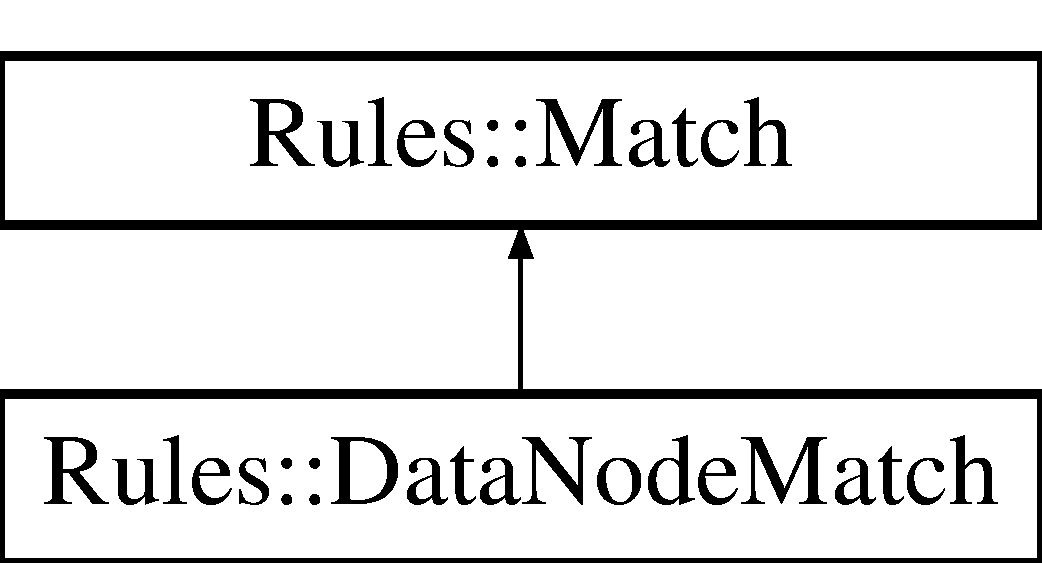
\includegraphics[height=2.000000cm]{structRules_1_1DataNodeMatch}
\end{center}
\end{figure}
\subsection*{Public Member Functions}
\begin{DoxyCompactItemize}
\item 
virtual bool \hyperlink{structRules_1_1DataNodeMatch_a9b30f5181bccbbac274f27f2a0c8421b}{matches} (const \hyperlink{classDatabase_1_1DataNode}{Database\+::\+Data\+Node} $\ast$database, void $\ast$bindings)
\begin{DoxyCompactList}\small\item\em Matches the given database by checking each element in the database against the matches\+Node method. \end{DoxyCompactList}\item 
bool \hyperlink{structRules_1_1DataNodeMatch_af96494dfe20521bc7a43eceac013d9c8}{matches\+Children} (const \hyperlink{classDatabase_1_1DataGroup}{Database\+::\+Data\+Group} $\ast$group, void $\ast$bindings)
\begin{DoxyCompactList}\small\item\em Matches all the children of the given group to see if any of them pass the matches\+Node test. This is used in the implementation of the matches method to iterate through items in the database. \end{DoxyCompactList}\item 
virtual bool \hyperlink{structRules_1_1DataNodeMatch_a9b2515abf3ef2b216cfc4ea18e95e07d}{matches\+Node} (const \hyperlink{classDatabase_1_1DataNode}{Database\+::\+Data\+Node} $\ast$node, void $\ast$bindings)=0
\begin{DoxyCompactList}\small\item\em Matches the data node from the database against the criteria in this match. \end{DoxyCompactList}\end{DoxyCompactItemize}
\subsection*{Public Attributes}
\begin{DoxyCompactItemize}
\item 
\hyperlink{structRules_1_1DataNodeMatch}{Data\+Node\+Match} $\ast$ \hyperlink{structRules_1_1DataNodeMatch_a6a55cae5c9f132912f877f34b8fa716e}{right\+Sibling}\hypertarget{structRules_1_1DataNodeMatch_a6a55cae5c9f132912f877f34b8fa716e}{}\label{structRules_1_1DataNodeMatch_a6a55cae5c9f132912f877f34b8fa716e}

\begin{DoxyCompactList}\small\item\em The right sibling of this node in match tree. \end{DoxyCompactList}\end{DoxyCompactItemize}


\subsection{Detailed Description}
A struct derived from \hyperlink{structRules_1_1Match}{Match}, it is responsible for matching a single Data\+Node in the database. 

Conceptually, the match class could match the whole database in a single operation\+: it is only ever fed the whole database, so it can do with that what it likes. However in practical, the vast majority of matching requirements involve trying to find a single item in the database. This struct\textquotesingle{}s match method iterates through the items in the database, and calls matches\+Node on each one. Matches items can be implemented in sub-\/classes to check if the item fulfils the mtach criteria.

Data node matches are arranged into tree, just like how data nodes are.

\begin{DoxySeeAlso}{See also}
\hyperlink{structRules_1_1Match}{Match} 
\end{DoxySeeAlso}


\subsection{Member Function Documentation}
\index{Rules\+::\+Data\+Node\+Match@{Rules\+::\+Data\+Node\+Match}!matches@{matches}}
\index{matches@{matches}!Rules\+::\+Data\+Node\+Match@{Rules\+::\+Data\+Node\+Match}}
\subsubsection[{\texorpdfstring{matches(const Database\+::\+Data\+Node $\ast$database, void $\ast$bindings)}{matches(const Database::DataNode *database, void *bindings)}}]{\setlength{\rightskip}{0pt plus 5cm}bool Rules\+::\+Data\+Node\+Match\+::matches (
\begin{DoxyParamCaption}
\item[{const {\bf Database\+::\+Data\+Node} $\ast$}]{database, }
\item[{void $\ast$}]{bindings}
\end{DoxyParamCaption}
)\hspace{0.3cm}{\ttfamily [virtual]}}\hypertarget{structRules_1_1DataNodeMatch_a9b30f5181bccbbac274f27f2a0c8421b}{}\label{structRules_1_1DataNodeMatch_a9b30f5181bccbbac274f27f2a0c8421b}


Matches the given database by checking each element in the database against the matches\+Node method. 


\begin{DoxyParams}{Parameters}
{\em database} & The database to match on. \\
\hline
{\em bindings} & When part of the if clause matches a wild card, it is added to the bindings. This parameter is both input and output parameter. \\
\hline
\end{DoxyParams}
\begin{DoxyReturn}{Returns}
true if matches, else returns false. 
\end{DoxyReturn}


Implements \hyperlink{structRules_1_1Match_a41fdfdc0b535e029369be3e18854e14e}{Rules\+::\+Match}.

\index{Rules\+::\+Data\+Node\+Match@{Rules\+::\+Data\+Node\+Match}!matches\+Children@{matches\+Children}}
\index{matches\+Children@{matches\+Children}!Rules\+::\+Data\+Node\+Match@{Rules\+::\+Data\+Node\+Match}}
\subsubsection[{\texorpdfstring{matches\+Children(const Database\+::\+Data\+Group $\ast$group, void $\ast$bindings)}{matchesChildren(const Database::DataGroup *group, void *bindings)}}]{\setlength{\rightskip}{0pt plus 5cm}bool Rules\+::\+Data\+Node\+Match\+::matches\+Children (
\begin{DoxyParamCaption}
\item[{const {\bf Database\+::\+Data\+Group} $\ast$}]{group, }
\item[{void $\ast$}]{bindings}
\end{DoxyParamCaption}
)}\hypertarget{structRules_1_1DataNodeMatch_af96494dfe20521bc7a43eceac013d9c8}{}\label{structRules_1_1DataNodeMatch_af96494dfe20521bc7a43eceac013d9c8}


Matches all the children of the given group to see if any of them pass the matches\+Node test. This is used in the implementation of the matches method to iterate through items in the database. 


\begin{DoxyParams}{Parameters}
{\em group} & The group to match on. \\
\hline
{\em bindings} & When part of the if clause matches a wild card, it is added to the bindings. This parameter is both input and output parameter. \\
\hline
\end{DoxyParams}
\begin{DoxyReturn}{Returns}
true if matches, else return false. 
\end{DoxyReturn}
\index{Rules\+::\+Data\+Node\+Match@{Rules\+::\+Data\+Node\+Match}!matches\+Node@{matches\+Node}}
\index{matches\+Node@{matches\+Node}!Rules\+::\+Data\+Node\+Match@{Rules\+::\+Data\+Node\+Match}}
\subsubsection[{\texorpdfstring{matches\+Node(const Database\+::\+Data\+Node $\ast$node, void $\ast$bindings)=0}{matchesNode(const Database::DataNode *node, void *bindings)=0}}]{\setlength{\rightskip}{0pt plus 5cm}virtual bool Rules\+::\+Data\+Node\+Match\+::matches\+Node (
\begin{DoxyParamCaption}
\item[{const {\bf Database\+::\+Data\+Node} $\ast$}]{node, }
\item[{void $\ast$}]{bindings}
\end{DoxyParamCaption}
)\hspace{0.3cm}{\ttfamily [pure virtual]}}\hypertarget{structRules_1_1DataNodeMatch_a9b2515abf3ef2b216cfc4ea18e95e07d}{}\label{structRules_1_1DataNodeMatch_a9b2515abf3ef2b216cfc4ea18e95e07d}


Matches the data node from the database against the criteria in this match. 


\begin{DoxyParams}{Parameters}
{\em node} & The database to match on. \\
\hline
{\em bindings} & When part of the if clause matches a wild card, it is added to the bindings. This parameter is both input and output parameter. \\
\hline
\end{DoxyParams}
\begin{DoxyReturn}{Returns}
true if matches, else return false. 
\end{DoxyReturn}


The documentation for this struct was generated from the following files\+:\begin{DoxyCompactItemize}
\item 
Engine/\+Rules/Data\+Node\+Match.\+h\item 
Engine/\+Rules/Data\+Node\+Match.\+cpp\end{DoxyCompactItemize}

\hypertarget{classDatabase_1_1Datum}{}\section{Database\+:\+:Datum$<$ T $>$ Class Template Reference}
\label{classDatabase_1_1Datum}\index{Database\+::\+Datum$<$ T $>$@{Database\+::\+Datum$<$ T $>$}}


A \hyperlink{classDatabase_1_1Datum}{Datum} consists of an identifier and and value. In \hyperlink{namespaceDatabase}{Database}\textquotesingle{}s tree structure, a leaf node is a \hyperlink{classDatabase_1_1Datum}{Datum}.  




{\ttfamily \#include $<$Datum.\+h$>$}

Inheritance diagram for Database\+:\+:Datum$<$ T $>$\+:\begin{figure}[H]
\begin{center}
\leavevmode
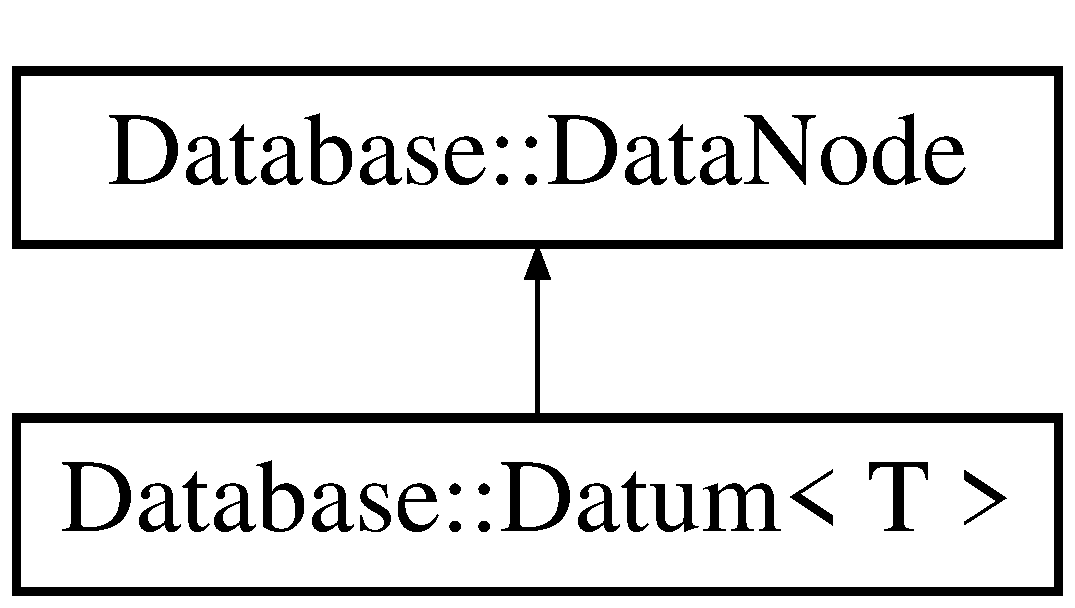
\includegraphics[height=2.000000cm]{classDatabase_1_1Datum}
\end{center}
\end{figure}
\subsection*{Public Member Functions}
\begin{DoxyCompactItemize}
\item 
\hyperlink{classDatabase_1_1Datum_a6c8c58a7e440ababc4f0a87f5da4d387}{Datum} (T value)
\begin{DoxyCompactList}\small\item\em \hyperlink{classDatabase_1_1Datum}{Datum} constructor. \end{DoxyCompactList}\item 
\hyperlink{classDatabase_1_1Datum_a7e35720d2b0b7baaff936163314940dd}{Datum} (const std\+::string \&\hyperlink{classDatabase_1_1DataNode_a2417b60924a11cf9157b996fbf7b2ca5}{identifier}, \hyperlink{classDatabase_1_1DataNode}{Data\+Node} $\ast$\hyperlink{classDatabase_1_1DataNode_ae335fc33c3813e8a6638d50faef44d5d}{right\+Sibling}, T value)
\begin{DoxyCompactList}\small\item\em \hyperlink{classDatabase_1_1Datum}{Datum} constructor. \end{DoxyCompactList}\item 
virtual \hyperlink{classDatabase_1_1Datum_a973e321d98f8be376fd8ec772446f480}{$\sim$\+Datum} ()\hypertarget{classDatabase_1_1Datum_a973e321d98f8be376fd8ec772446f480}{}\label{classDatabase_1_1Datum_a973e321d98f8be376fd8ec772446f480}

\begin{DoxyCompactList}\small\item\em $\sim$\+Datum destructor \end{DoxyCompactList}\item 
void \hyperlink{classDatabase_1_1Datum_a636a8ed59bfcb2947100f8181a9b5c73}{set\+Value} (T new\+Value)
\begin{DoxyCompactList}\small\item\em To change the value of the \hyperlink{classDatabase_1_1Datum}{Datum}. \end{DoxyCompactList}\item 
T \hyperlink{classDatabase_1_1Datum_ae33499d38a1e3ab4725fbf4f3ba9c284}{get\+Value} () const 
\begin{DoxyCompactList}\small\item\em To get the value of the \hyperlink{classDatabase_1_1Datum}{Datum}. \end{DoxyCompactList}\item 
bool \hyperlink{classDatabase_1_1Datum_a81a243020da7294ad331b50d45b86ad8}{is\+Datum} ()
\begin{DoxyCompactList}\small\item\em Allows user to check whether this node is a \hyperlink{classDatabase_1_1Datum}{Datum} or not. \end{DoxyCompactList}\end{DoxyCompactItemize}
\subsection*{Additional Inherited Members}


\subsection{Detailed Description}
\subsubsection*{template$<$class T$>$\\*
class Database\+::\+Datum$<$ T $>$}

A \hyperlink{classDatabase_1_1Datum}{Datum} consists of an identifier and and value. In \hyperlink{namespaceDatabase}{Database}\textquotesingle{}s tree structure, a leaf node is a \hyperlink{classDatabase_1_1Datum}{Datum}. 

\begin{DoxySeeAlso}{See also}
\hyperlink{classDatabase_1_1DataNode}{Data\+Node} 

\hyperlink{classDatabase_1_1DataGroup}{Data\+Group} 
\end{DoxySeeAlso}


\subsection{Constructor \& Destructor Documentation}
\index{Database\+::\+Datum@{Database\+::\+Datum}!Datum@{Datum}}
\index{Datum@{Datum}!Database\+::\+Datum@{Database\+::\+Datum}}
\subsubsection[{\texorpdfstring{Datum(\+T value)}{Datum(T value)}}]{\setlength{\rightskip}{0pt plus 5cm}template$<$class T $>$ {\bf Database\+::\+Datum}$<$ T $>$\+::{\bf Datum} (
\begin{DoxyParamCaption}
\item[{T}]{value}
\end{DoxyParamCaption}
)}\hypertarget{classDatabase_1_1Datum_a6c8c58a7e440ababc4f0a87f5da4d387}{}\label{classDatabase_1_1Datum_a6c8c58a7e440ababc4f0a87f5da4d387}


\hyperlink{classDatabase_1_1Datum}{Datum} constructor. 


\begin{DoxyParams}{Parameters}
{\em value} & the value that the \hyperlink{classDatabase_1_1Datum}{Datum} holds. \\
\hline
\end{DoxyParams}
\index{Database\+::\+Datum@{Database\+::\+Datum}!Datum@{Datum}}
\index{Datum@{Datum}!Database\+::\+Datum@{Database\+::\+Datum}}
\subsubsection[{\texorpdfstring{Datum(const std\+::string \&identifier, Data\+Node $\ast$right\+Sibling, T value)}{Datum(const std::string &identifier, DataNode *rightSibling, T value)}}]{\setlength{\rightskip}{0pt plus 5cm}template$<$class T $>$ {\bf Database\+::\+Datum}$<$ T $>$\+::{\bf Datum} (
\begin{DoxyParamCaption}
\item[{const std\+::string \&}]{identifier, }
\item[{{\bf Data\+Node} $\ast$}]{right\+Sibling, }
\item[{T}]{value}
\end{DoxyParamCaption}
)}\hypertarget{classDatabase_1_1Datum_a7e35720d2b0b7baaff936163314940dd}{}\label{classDatabase_1_1Datum_a7e35720d2b0b7baaff936163314940dd}


\hyperlink{classDatabase_1_1Datum}{Datum} constructor. 


\begin{DoxyParams}{Parameters}
{\em identifier} & a string parameter. \\
\hline
{\em right\+Sibling} & a \hyperlink{classDatabase_1_1DataNode}{Data\+Node} pointer representing this node\textquotesingle{}s right sibling in tree. \\
\hline
{\em value} & the value that the \hyperlink{classDatabase_1_1Datum}{Datum} holds. \\
\hline
\end{DoxyParams}


\subsection{Member Function Documentation}
\index{Database\+::\+Datum@{Database\+::\+Datum}!get\+Value@{get\+Value}}
\index{get\+Value@{get\+Value}!Database\+::\+Datum@{Database\+::\+Datum}}
\subsubsection[{\texorpdfstring{get\+Value() const }{getValue() const }}]{\setlength{\rightskip}{0pt plus 5cm}template$<$class T $>$ T {\bf Database\+::\+Datum}$<$ T $>$\+::get\+Value (
\begin{DoxyParamCaption}
{}
\end{DoxyParamCaption}
) const}\hypertarget{classDatabase_1_1Datum_ae33499d38a1e3ab4725fbf4f3ba9c284}{}\label{classDatabase_1_1Datum_ae33499d38a1e3ab4725fbf4f3ba9c284}


To get the value of the \hyperlink{classDatabase_1_1Datum}{Datum}. 

\begin{DoxyReturn}{Returns}
The value that the datum is currently holding. 
\end{DoxyReturn}
\index{Database\+::\+Datum@{Database\+::\+Datum}!is\+Datum@{is\+Datum}}
\index{is\+Datum@{is\+Datum}!Database\+::\+Datum@{Database\+::\+Datum}}
\subsubsection[{\texorpdfstring{is\+Datum()}{isDatum()}}]{\setlength{\rightskip}{0pt plus 5cm}template$<$class T $>$ bool {\bf Database\+::\+Datum}$<$ T $>$\+::is\+Datum (
\begin{DoxyParamCaption}
{}
\end{DoxyParamCaption}
)}\hypertarget{classDatabase_1_1Datum_a81a243020da7294ad331b50d45b86ad8}{}\label{classDatabase_1_1Datum_a81a243020da7294ad331b50d45b86ad8}


Allows user to check whether this node is a \hyperlink{classDatabase_1_1Datum}{Datum} or not. 

\begin{DoxyReturn}{Returns}
true if this node is a \hyperlink{classDatabase_1_1Datum}{Datum}, otherwise returns false. 
\end{DoxyReturn}
\index{Database\+::\+Datum@{Database\+::\+Datum}!set\+Value@{set\+Value}}
\index{set\+Value@{set\+Value}!Database\+::\+Datum@{Database\+::\+Datum}}
\subsubsection[{\texorpdfstring{set\+Value(\+T new\+Value)}{setValue(T newValue)}}]{\setlength{\rightskip}{0pt plus 5cm}template$<$class T $>$ void {\bf Database\+::\+Datum}$<$ T $>$\+::set\+Value (
\begin{DoxyParamCaption}
\item[{T}]{new\+Value}
\end{DoxyParamCaption}
)}\hypertarget{classDatabase_1_1Datum_a636a8ed59bfcb2947100f8181a9b5c73}{}\label{classDatabase_1_1Datum_a636a8ed59bfcb2947100f8181a9b5c73}


To change the value of the \hyperlink{classDatabase_1_1Datum}{Datum}. 


\begin{DoxyParams}{Parameters}
{\em new\+Value} & The new value that is going to be assigned to the \hyperlink{classDatabase_1_1Datum}{Datum}. \\
\hline
\end{DoxyParams}


The documentation for this class was generated from the following files\+:\begin{DoxyCompactItemize}
\item 
Engine/\+Database/Datum.\+h\item 
Engine/\+Database/Datum.\+cpp\end{DoxyCompactItemize}

\hypertarget{structRules_1_1Match}{}\section{Rules\+:\+:Match Struct Reference}
\label{structRules_1_1Match}\index{Rules\+::\+Match@{Rules\+::\+Match}}


Provides the mechanism to match the data item from the rule with any item inside the database.  




{\ttfamily \#include $<$Match.\+h$>$}

\subsection*{Public Member Functions}
\begin{DoxyCompactItemize}
\item 
virtual bool \hyperlink{structRules_1_1Match_a41fdfdc0b535e029369be3e18854e14e}{matches} (const \hyperlink{classDatabase_1_1DataNode}{Database\+::\+Data\+Node} $\ast$database, void $\ast$bindings)=0
\begin{DoxyCompactList}\small\item\em Check the match on the database. \end{DoxyCompactList}\end{DoxyCompactItemize}


\subsection{Detailed Description}
Provides the mechanism to match the data item from the rule with any item inside the database. 

\subsection{Member Function Documentation}
\index{Rules\+::\+Match@{Rules\+::\+Match}!matches@{matches}}
\index{matches@{matches}!Rules\+::\+Match@{Rules\+::\+Match}}
\subsubsection[{\texorpdfstring{matches(const Database\+::\+Data\+Node $\ast$database, void $\ast$bindings)=0}{matches(const Database::DataNode *database, void *bindings)=0}}]{\setlength{\rightskip}{0pt plus 5cm}virtual bool Rules\+::\+Match\+::matches (
\begin{DoxyParamCaption}
\item[{const {\bf Database\+::\+Data\+Node} $\ast$}]{database, }
\item[{void $\ast$}]{bindings}
\end{DoxyParamCaption}
)\hspace{0.3cm}{\ttfamily [pure virtual]}}\hypertarget{structRules_1_1Match_a41fdfdc0b535e029369be3e18854e14e}{}\label{structRules_1_1Match_a41fdfdc0b535e029369be3e18854e14e}


Check the match on the database. 


\begin{DoxyParams}{Parameters}
{\em database} & The database to match on. \\
\hline
{\em bindings} & When part of the if clause matches a wild card, it is added to the bindings. This parameter is both input and output parameter. \\
\hline
\end{DoxyParams}
\begin{DoxyReturn}{Returns}
true if matches, else returns false. 
\end{DoxyReturn}


The documentation for this struct was generated from the following file\+:\begin{DoxyCompactItemize}
\item 
Engine/\+Rules/Match.\+h\end{DoxyCompactItemize}

\hypertarget{classRules_1_1Rule}{}\section{Rules\+:\+:Rule Class Reference}
\label{classRules_1_1Rule}\index{Rules\+::\+Rule@{Rules\+::\+Rule}}


Represent a rule in a Rule-\/based system. A rule has two components\+: an if clause is going to be used to match against the database and a function to perform any action required.  




{\ttfamily \#include $<$Rule.\+h$>$}

\subsection*{Public Member Functions}
\begin{DoxyCompactItemize}
\item 
virtual void \hyperlink{classRules_1_1Rule_a6fe9b4fa6aaface7ba7f2400d2b27dbc}{action} ()=0
\begin{DoxyCompactList}\small\item\em The action is going to be carried out when the rule matches. \end{DoxyCompactList}\end{DoxyCompactItemize}
\subsection*{Public Attributes}
\begin{DoxyCompactItemize}
\item 
\hyperlink{structRules_1_1Match}{Match} $\ast$ \hyperlink{classRules_1_1Rule_a4b4030afd5ca2d4812ba9100b3b0047d}{if\+Clause}\hypertarget{classRules_1_1Rule_a4b4030afd5ca2d4812ba9100b3b0047d}{}\label{classRules_1_1Rule_a4b4030afd5ca2d4812ba9100b3b0047d}

\begin{DoxyCompactList}\small\item\em Consist of a set of data items, in a similar format to those in the database. \end{DoxyCompactList}\end{DoxyCompactItemize}


\subsection{Detailed Description}
Represent a rule in a Rule-\/based system. A rule has two components\+: an if clause is going to be used to match against the database and a function to perform any action required. 

\subsection{Member Function Documentation}
\index{Rules\+::\+Rule@{Rules\+::\+Rule}!action@{action}}
\index{action@{action}!Rules\+::\+Rule@{Rules\+::\+Rule}}
\subsubsection[{\texorpdfstring{action()=0}{action()=0}}]{\setlength{\rightskip}{0pt plus 5cm}virtual void Rules\+::\+Rule\+::action (
\begin{DoxyParamCaption}
{}
\end{DoxyParamCaption}
)\hspace{0.3cm}{\ttfamily [pure virtual]}}\hypertarget{classRules_1_1Rule_a6fe9b4fa6aaface7ba7f2400d2b27dbc}{}\label{classRules_1_1Rule_a6fe9b4fa6aaface7ba7f2400d2b27dbc}


The action is going to be carried out when the rule matches. 

\begin{DoxyRefDesc}{Todo}
\item[\hyperlink{todo__todo000004}{Todo}]Examine the performance and reusability of using a method. If it is hard to expand, find a way to use a struct/class instead. \end{DoxyRefDesc}


The documentation for this class was generated from the following file\+:\begin{DoxyCompactItemize}
\item 
Engine/\+Rules/Rule.\+h\end{DoxyCompactItemize}

%--- End generated contents ---

% Index
\backmatter
\newpage
\phantomsection
\clearemptydoublepage
\addcontentsline{toc}{chapter}{Index}
\printindex

\end{document}
